\documentclass[journal,12pt,onecolumn]{IEEEtran}
\usepackage[utf8]{inputenc}   % Codificación de entrada
\usepackage[T1]{fontenc}      % Codificación de fuente
\usepackage[spanish,es-tabla]{babel}   % Idioma español
\usepackage{lmodern}          % Fuente moderna
\usepackage{amsmath, amssymb} % Matemáticas y símbolos
\usepackage{graphicx} 		  % Gráficos e imágenes
\graphicspath{{img/}{tablas/}{portada/}}  % Las imágenes se buscarán en la carpeta "img"
\usepackage{longtable}      % Para tablas que se extienden en varias páginas
\usepackage{tabularx}	% Tablas avanzadas
\usepackage{threeparttable}
\usepackage{hyperref}	% Hipervínculos

%-------------------------------------------
% Otros paquetes útiles (personaliza según tus necesidades)
%-------------------------------------------
\usepackage{caption}
\usepackage{subcaption}
\usepackage{xcolor}
\usepackage{setspace}

%-------------------------------------------
% Comandos personalizados
\renewcommand{\listtablename}{Índice de tablas}
\renewcommand{\appendixname}{Anexos}
\definecolor{colorreferences}{RGB}{48,134,3}

% Metadatos del PDF
\hypersetup{
	unicode=true,
	hidelinks,
	colorlinks=true,       % false: boxed links; true: colored links
	linkcolor=black,          % color of internal links (change box color with linkbordercolor)
	citecolor=colorreferences,        % color of links to bibliography
	filecolor=magenta,      % color of file links
	urlcolor=blue,           % color of external links
	linkbordercolor={0 0 0}
}
%-------------------------------------------
% Inicio del documento
%-------------------------------------------
\begin{document}

% Aquí se encuentra el archivo con la portada
\begin{titlepage}
	\centering
	%-------------------------------------------
	% Logos en una tabla: izquierda, centro y derecha
	\begin{tabular}{@{}p{0.3\textwidth} p{0.3\textwidth} p{0.3\textwidth}@{}}
		
\includegraphics[height=2cm]{tecnm} & 
		\centering 
\includegraphics[height=1.5cm]{SEP} & 
		\raggedleft 
\includegraphics[height=2cm]{ith.jpg} \\
	\end{tabular}
	
	\vspace{2em}
	
	\noindent
	%-------------------------------------------
	%	Información institucional y académica (esquina superior izquierda)
	\begin{minipage}[t]{0.6\textwidth}
		\raggedright
		\small \textbf{%
			Instituto Tecnológico de Hermosillo\\
			Materia: Robótica\\
			Profesor: Medina Gil Lamadrid, Jesús Iván%
		}
	\end{minipage}%
	\hfill
	%	fecha actual (esquina superior derecha), en letras pequeñas y en negrita.
	\begin{minipage}[t]{0.3\textwidth}
		\raggedleft
		\small \textbf{\today}
	\end{minipage}
	
	\vspace{2em}
	
	%-----------------------------------------
	% Unidad y Título de la tarea en letras grandes y en negrita
%	{\large \textbf{Unidad Final}}\\
	{\Huge \textbf{Reporte final del Robot}}
		
	\vspace{1em}
	
	%---------------------------------------
	% Tabla con la información del equipo
	%---------------------------------------
	% Encabezado del equipo
	\begin{center}
		{\Large \textbf{Equipo 5}}
		
		{\small \textbf{https://github.com/JesusLazar/Robotica.git}}
	\end{center}
	
	\vspace{1em}
	
	% Tabla de integrantes:
	% Cada fila contiene: foto (columna izquierda) y datos del integrante (columna derecha)
	\begin{center}
		\begin{tabular}{c c}
			\begin{tabular}{c}
			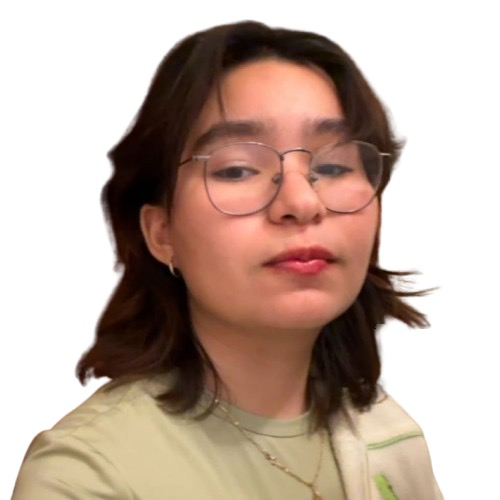
\includegraphics[height=3cm]{Mich.jpg} \\
				\textbf{Arvizu, }\\ Michelle \\ \texttt{l21330532@hermosillo.tecnm.mx } \\ Teléfono: (6221164719)
			\end{tabular} &
			\begin{tabular}{c}
				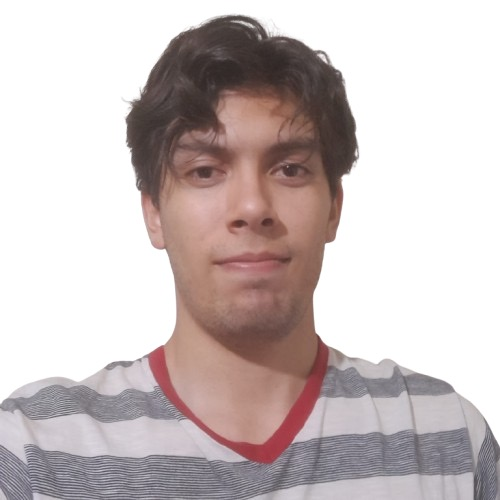
\includegraphics[height=3cm]{Lazaro.jpg} \\
				\textbf{Carranza,}\\ Jesús \\ \texttt{l21330548@hermosillo.tecnm.mx} \\ Teléfono: (6621130410)
			\end{tabular} \\ \vspace{2em}
			\begin{tabular}{c}
				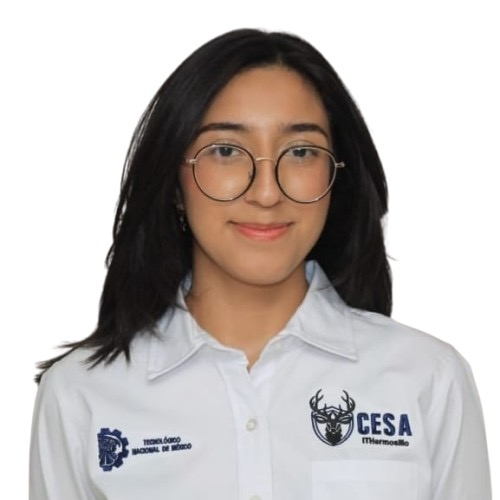
\includegraphics[height=3cm]{Morelia.jpg} \\
				\textbf{Montoya,}\\ Morelia \\ \texttt{l21330642@hermosillo.tecnm.mx} \\ Teléfono: (6624251581)
			\end{tabular} &
			\begin{tabular}{c}
				\includegraphics[height=3cm]{Anitafoto.jpg} \\
				\textbf{Moreno,}\\ Ana \\ \texttt{l21330650@hermosillo.tecnm.mx} \\ Teléfono: (6624591969)
			\end{tabular}
		\end{tabular}
	\end{center}

\end{titlepage}

%	Es innecesario poner el índice porque ya aparece en los marcadores del PDF
%\tableofcontents

% Ejemplo de inclusión de una sección (por ejemplo, "introduccion.tex" debe estar en la carpeta "secciones" y se recomienda no usar carácteres especiales (tilde) o espacios)
\section{Introducción}

Los sensores son componentes críticos en los sistemas robóticos, ya que permiten a los robots percibir y responder a su entorno. Estos dispositivos se clasifican en dos categorías principales: \textbf{sensores internos} y \textbf{sensores externos}. Los sensores internos se utilizan para monitorear el estado interno del robot, como su posición, velocidad, aceleración y fuerzas aplicadas. Por otro lado, los sensores externos permiten al robot interactuar con su entorno, detectando objetos, obstáculos y otras características relevantes \cite{UAEMex}.

En robótica, los sensores internos son esenciales para el control y la navegación, ya que proporcionan información en tiempo real sobre el estado del robot. Esta información es utilizada por el controlador para tomar decisiones y generar comandos de control. Por ejemplo, los encoders y potenciómetros son ampliamente utilizados para medir la posición, mientras que los tacómetros y sensores de efecto Hall se emplean para medir la velocidad \cite{OMCH, EfectoHall}.

En esta sección, se describen los principales tipos de sensores internos utilizados en robótica, incluyendo sensores de posición, velocidad, aceleración y fuerza. Cada uno de estos sensores desempeña un papel crucial en el control y la navegación de los robots, permitiendo que estos sistemas operen de manera precisa y eficiente.


\section{Sensores}
Un sensor es un dispositivo que detecta el cambio en el entorno y responde a alguna salida en el otro sistema. Un sensor convierte un fenómeno físico en un voltaje analógico medible (o, a veces, una señal digital) convertido en una pantalla legible para humanos o transmitida para lectura o procesamiento adicional. 



\section{Sensores Internos}

Los sensores internos son dispositivos esenciales en los sistemas robóticos, ya que permiten monitorear el estado interno del robot, como su posición, velocidad, aceleración y fuerzas aplicadas. Estos sensores proporcionan información crítica que el controlador utiliza para tomar decisiones y generar comandos de control. Dependiendo de la cantidad física que miden, los sensores internos se clasifican en sensores de posición, velocidad, aceleración y fuerza.

\subsection{Sensores Internos de Posición}

Los sensores de posición son fundamentales para determinar la ubicación exacta de un robot o de sus componentes en un momento dado. Estos sensores son cruciales en aplicaciones que requieren precisión, como la manipulación de objetos o la navegación autónoma.

\subsubsection{Encoders}
El encoder es un dispositivo óptico digital que convierte el movimiento en una secuencia de pulsos digitales. Estos pulsos pueden ser contados o decodificados para obtener medidas relativas o absolutas de posición. Los encoders se clasifican en dos tipos principales: incrementales y absolutos. Además, pueden ser lineales o rotatorios, dependiendo de la aplicación \cite{OMCH}.

\begin{itemize}
	\item \textbf{Encoders incrementales}: Generan pulsos mientras se mueven, lo que permite medir la velocidad o la trayectoria de la posición. Sin embargo, no proporcionan información sobre la posición absoluta.
	\item \textbf{Encoders absolutos}: Generan una salida digital que indica directamente la posición actual, lo que los hace ideales para aplicaciones que requieren un conocimiento preciso de la posición inicial.
\end{itemize}

En la \autoref{fig:encoder} se muestra un ejemplo de este sensor.

\begin{figure}[h!]
	\centering
	\subfloat[Encoder]{%
		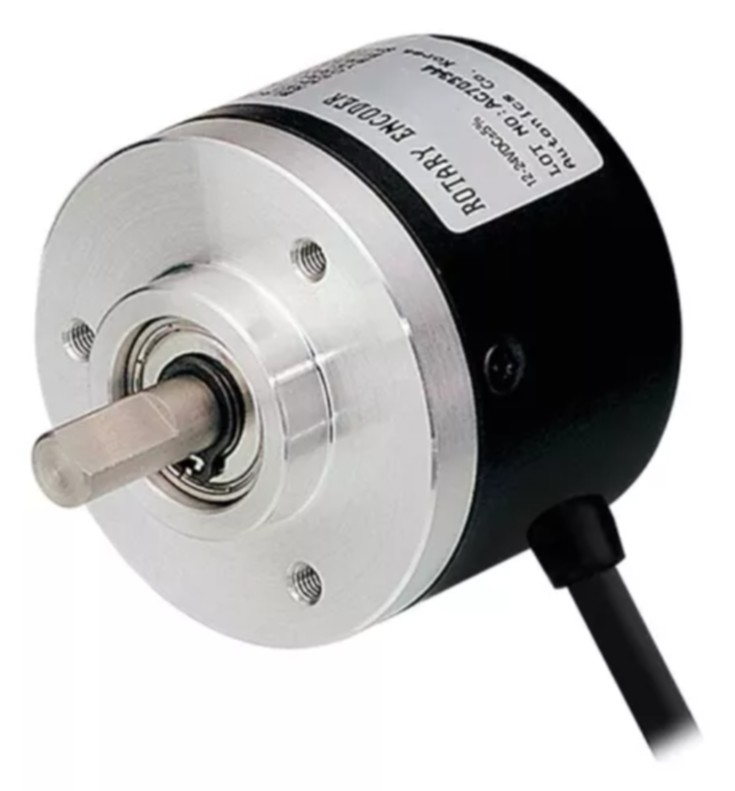
\includegraphics[width=0.2\textwidth]{encoder.jpg}%
		\label{fig:Encoder}
	}
	\subfloat[Encoder Funcionamiento]{%
		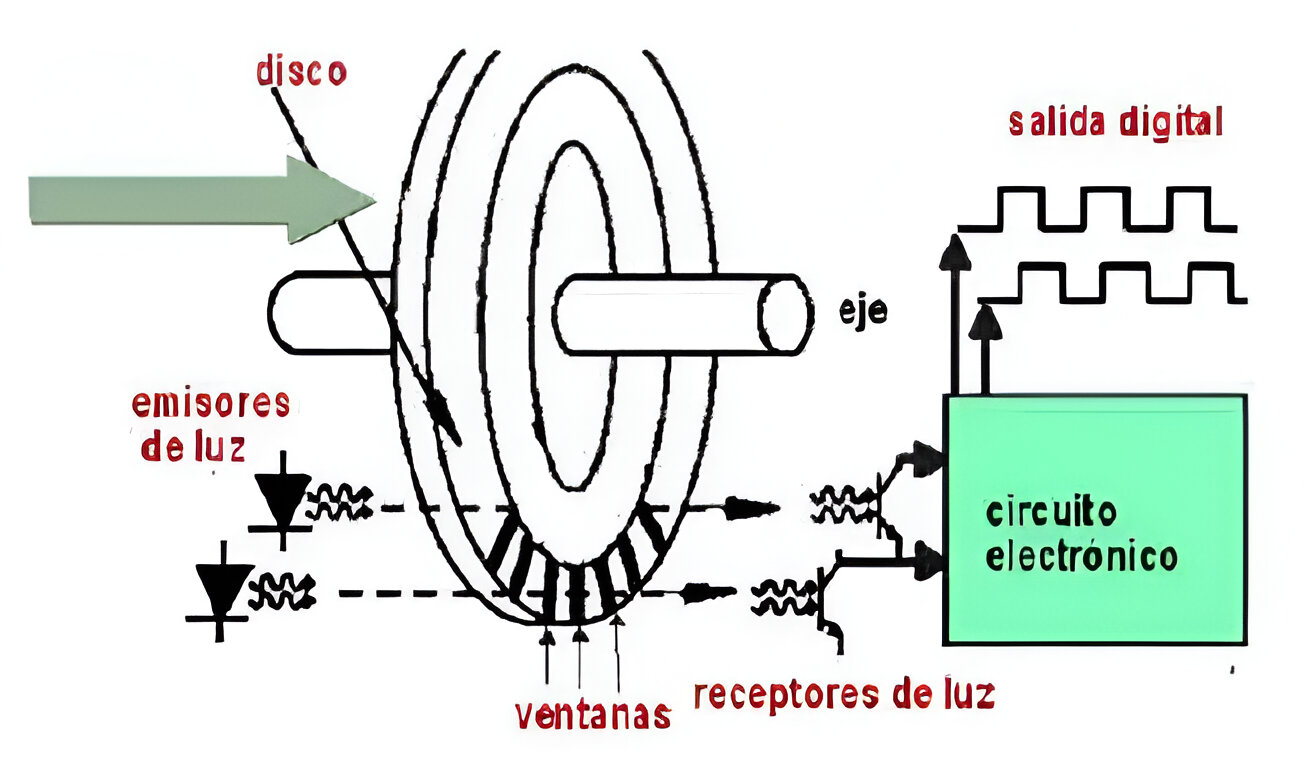
\includegraphics[width=0.35\textwidth]{img/encoder-fn}%
		\label{fig:encoder-fn}
	}
	\caption{Ejemplo de un encoder y su funcionamiento.}
	\label{fig:encoder}
\end{figure}

\subsubsection{Potenciómetro}
El potenciómetro es un sensor de posición que convierte desplazamientos lineales o angulares en una señal de voltaje. Consiste en una clavija deslizante que hace contacto con un elemento resistivo. A medida que el punto de contacto se mueve, la resistencia cambia en proporción al desplazamiento, lo que permite medir la posición. Los potenciómetros son ampliamente utilizados en aplicaciones de bajo costo y baja precisión \cite{Potenciometro}.

En la \autoref{fig:potenciometros} se muestra un ejemplo de este sensor.

\begin{figure}[h!]
	\centering
	\subfloat[Potenciómetro]{%
		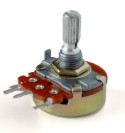
\includegraphics[width=0.2\textwidth]{potenciometro.jpg}%
		\label{fig:potenciometro}
	}
	\subfloat[Funcionamiento de potenciómetro]{%
		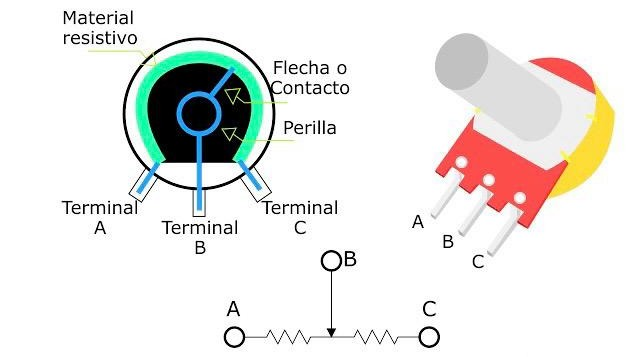
\includegraphics[width=0.3\textwidth]{img/potenciometro-funcionamiento}%
		\label{fig:potenciometro-funcionamiento}
	}
	\caption{Ejemplo de un potenciómetro y su funcionamiento.}
	\label{fig:potenciometros}
\end{figure}

\subsubsection{LVDT}
El transformador diferencial lineal variable (LVDT) es uno de los sensores de posición más precisos disponibles. Genera una señal de corriente alterna (CA) cuya magnitud está relacionada con el desplazamiento de un núcleo móvil. El LVDT es ideal para aplicaciones que requieren alta precisión y confiabilidad, como en la industria aeroespacial y médica \cite{LVDT}.

En la \autoref{fig:LVTD} se muestra un ejemplo de este sensor.

\begin{figure*}[h!]
	\centering
	\subfloat[Transformador diferencial lineal variable (LVDT)]{%
		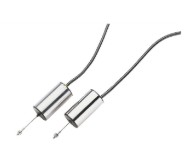
\includegraphics[width=0.2\textwidth]{lvtd.jpg}%
		\label{fig:lvdt}
	}
	\subfloat[Funcionamiento de un LVTD]{%
		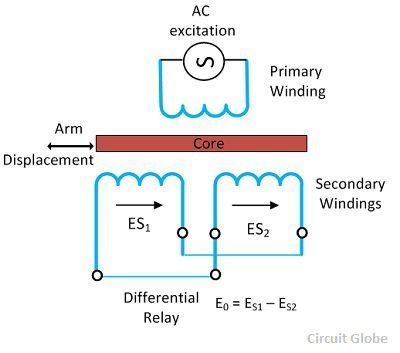
\includegraphics[width=0.2\textwidth]{img/lvdt-funcionamiento}%
		\label{fig:lvdt-funcionamiento}
	}
	\caption{Ejemplo de un LVDT y su funcionamiento.}
	\label{fig:LVTD}
\end{figure*}

\subsubsection{Sincronizadores y Resolvers}
Los sincronizadores y resolvers son sensores de posición que proporcionan señales analógicas como salida. A diferencia de los encoders, que producen señales digitales, estos dispositivos requieren un convertidor analógico-digital para procesar la señal. Son ampliamente utilizados en aplicaciones industriales y de automatización \cite{Resolver}.

En la \autoref{fig:resolver} se muestra un ejemplo de este sensor.
\begin{figure*}[h!]
	\centering
	\subfloat[Resolver]{%
		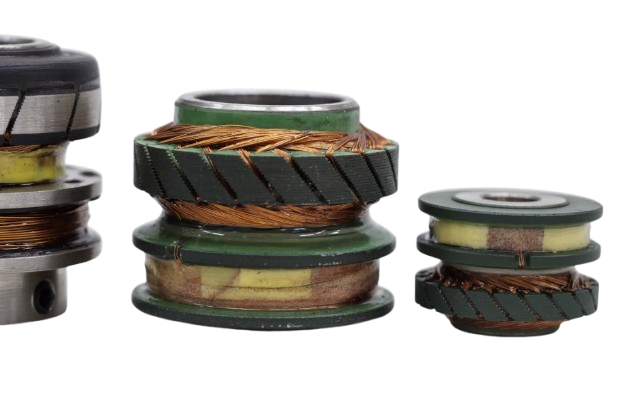
\includegraphics[width=0.3\textwidth]{img/resolvers-fn}%
		\label{fig:resolvers}
	}
	\subfloat[Funcionamiento de un LVTD]{%
		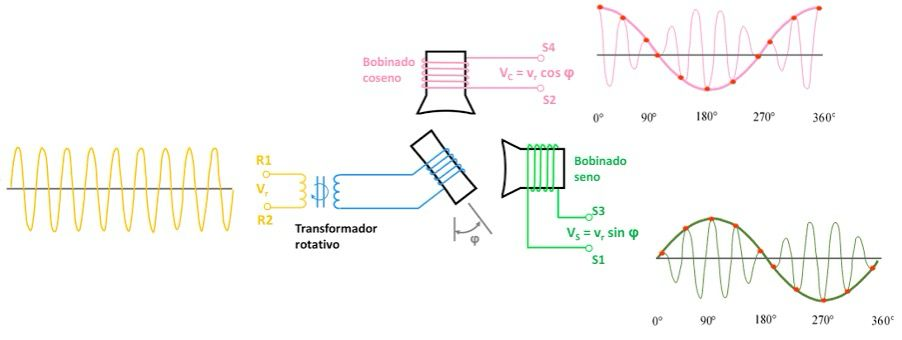
\includegraphics[width=0.5\textwidth]{img/resolvers-funcionamiento}%
		\label{fig:resolvers-funcionamiento}
	}
	\caption{Ejemplo de un resolver y su funcionamiento.}
	\label{fig:resolver}
\end{figure*}

\subsection{Sensores Internos de Velocidad}

Los sensores de velocidad son esenciales para controlar la dinámica de un robot, permitiendo medir la velocidad de rotación o traslación de sus componentes.

\subsubsection{Tacómetro}
El tacómetro es un sensor que mide directamente la velocidad de rotación de un eje. Funciona basándose en la regla de Fleming, que establece que el voltaje generado es proporcional a la velocidad de rotación. Los tacómetros son ampliamente utilizados en motores y sistemas de control de velocidad \cite{Acelerometro}.

En la \autoref{fig:tacometro2} se muestra un ejemplo de este sensor.

\begin{figure}[h!]
	\centering
	\subfloat[Tacómetro]{%
		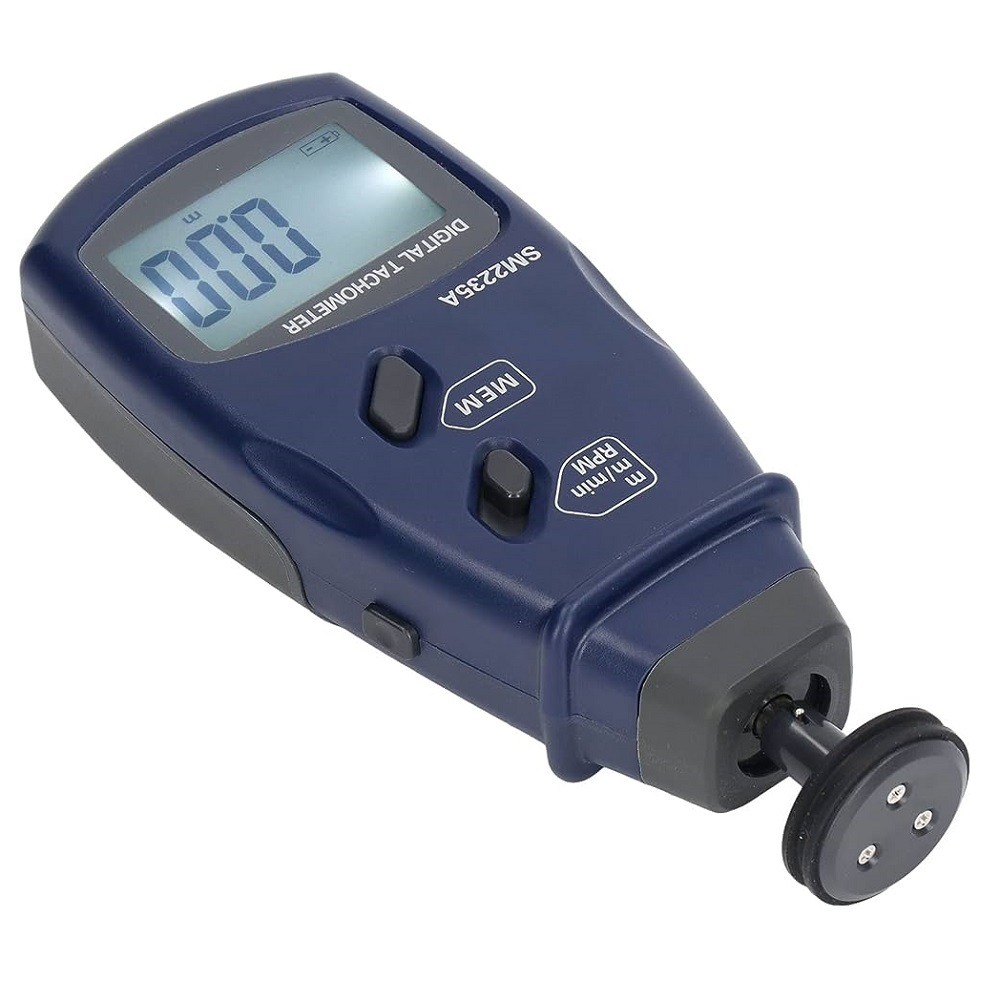
\includegraphics[width=0.2\textwidth]{img/tacometro}%
		\label{fig:tacometro}
	}
	\subfloat[Tacómetro Funcionamiento]{%
		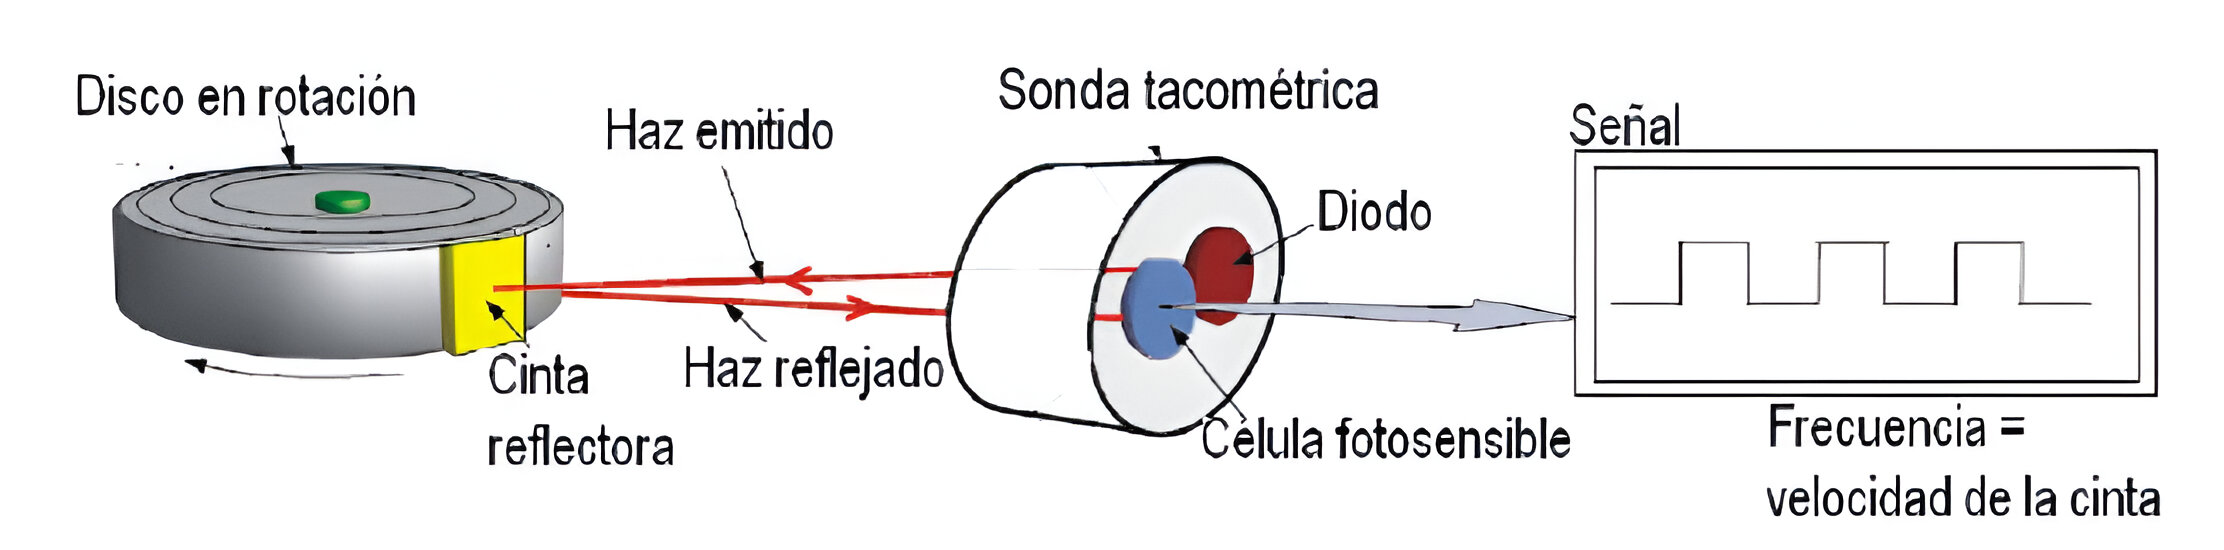
\includegraphics[width=0.7\textwidth]{img/tacometro-fn}%
		\label{fig:tacometro-fn}
	}
	\caption{Ejemplo de un tacómetro y su funcionamiento.}
	\label{fig:tacometro2}
\end{figure}

\subsubsection{Sensor de Efecto Hall}
El sensor de efecto Hall detecta campos magnéticos y convierte la velocidad de rotación de un imán en una señal eléctrica. Este tipo de sensor es ampliamente utilizado en aplicaciones automotrices e industriales debido a su alta precisión y durabilidad \cite{EfectoHall}.

En la \autoref{fig:SensordeEfectoHall} se muestra un ejemplo de este sensor.

\begin{figure}[h!]
	\centering
	\subfloat[Sensor de Efecto Hall]{%
		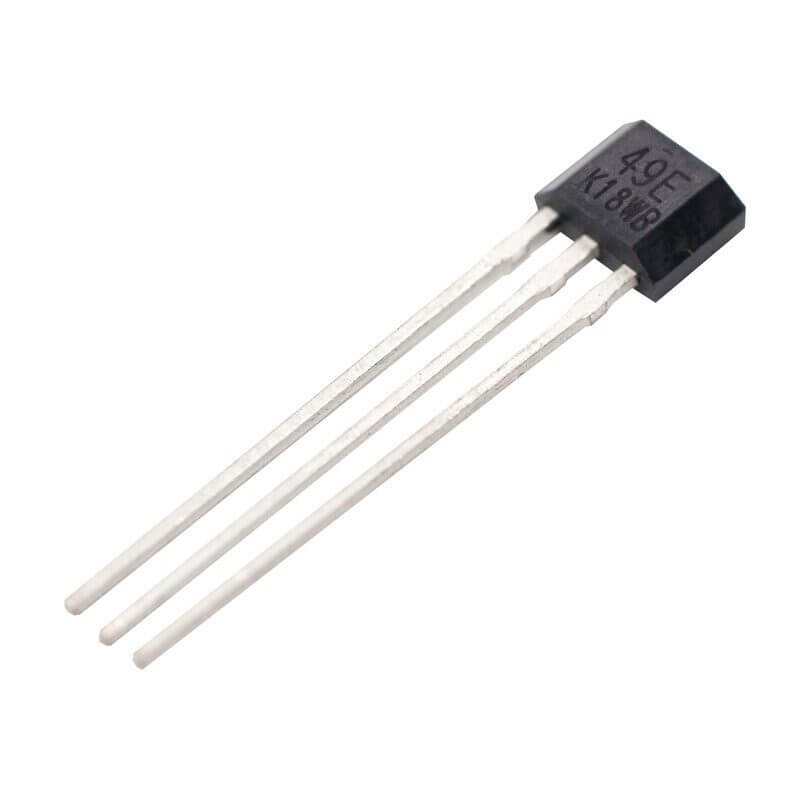
\includegraphics[width=0.2\textwidth]{img/Sensor_efecto_Hall}%
		\label{fig:Sensor_efecto_Hall}
	}
	\subfloat[Funcionamiento de Sensor de Efecto Hall]{%
		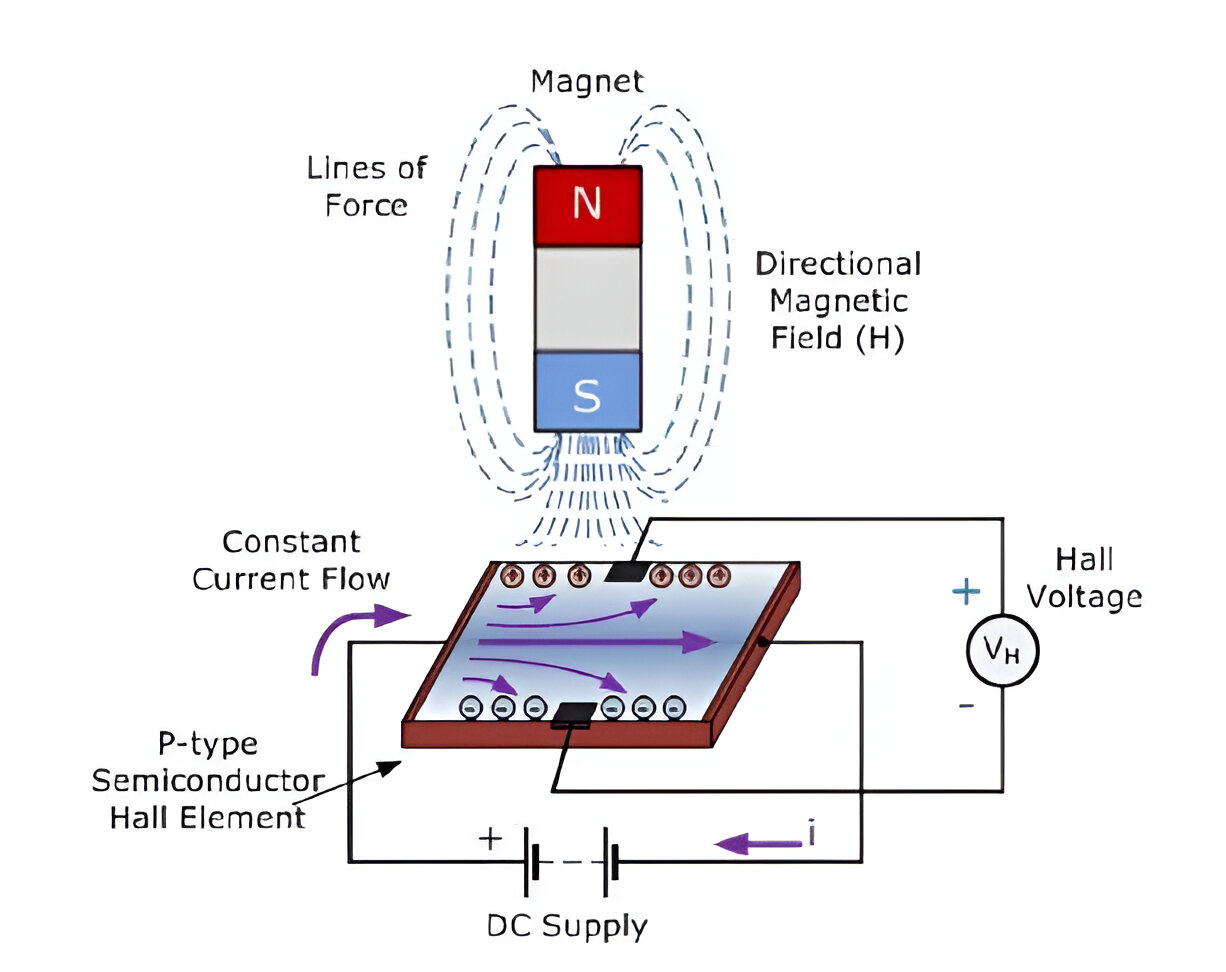
\includegraphics[width=0.35\textwidth]{img/Sensor_efecto_Hall-fn}%
		\label{fig:Sensor_efecto_Hall-fn}
	}
	\caption{Ejemplo de un sensor de efecto Hall y su funcionamiento.}
	\label{fig:SensordeEfectoHall}
\end{figure}

\section{Sensores Internos de Aceleración}

La aceleración es una medida crítica en sistemas robóticos, especialmente en aplicaciones que involucran movimientos rápidos o cambios bruscos de dirección. Los sensores de aceleración permiten medir esta cantidad física de manera directa, evitando la necesidad de calcularla a partir de datos de velocidad o posición, lo que puede ser computacionalmente costoso \cite{Acelerometro}.

\section{Sensores Internos de Fuerza}

Los sensores de fuerza, también conocidos como células de carga, son dispositivos que miden la fuerza aplicada sobre un objeto. Estos sensores son esenciales en aplicaciones como la manipulación de objetos, donde es necesario controlar la fuerza ejercida para evitar daños.

\subsection{Galgas Extensométricas}
Las galgas extensométricas son sensores que miden la deformación de un material, lo que permite calcular la fuerza aplicada. Estas galgas funcionan basándose en el principio de que la resistencia eléctrica de un conductor cambia cuando se estira o comprime \cite{Galgas}.

En la \autoref{fig:galgas} se muestra un ejemplo de este sensor.

\begin{figure*}[h!]
	\centering
	\subfloat[Imagen de Galgas Extensométricas]{%
		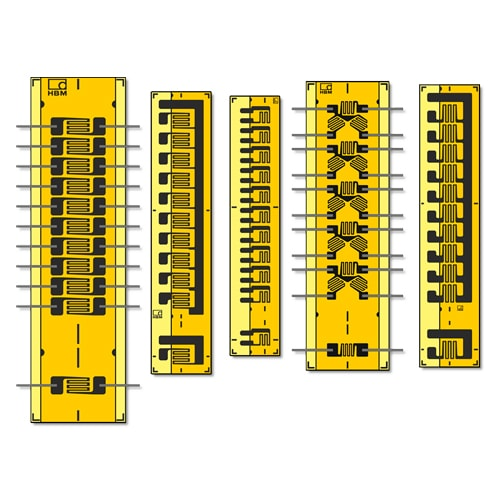
\includegraphics[width=0.25\textwidth]{img/Galgas_extensometricas}%
		\label{fig:galgas_extensometricas}
	}
	\subfloat[Funcionamiento de Galgas Extensométricas]{%
		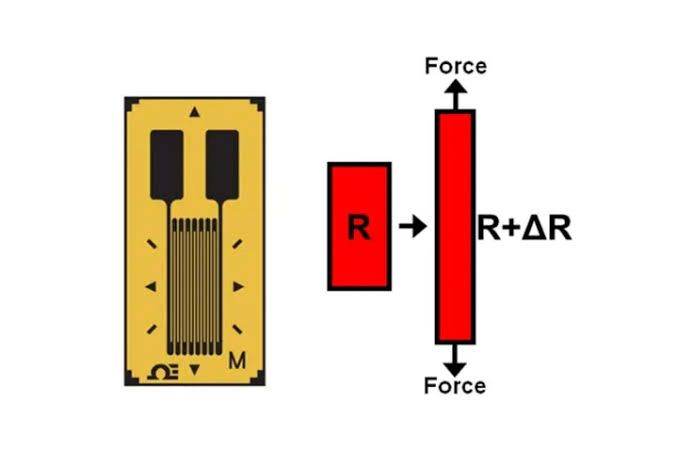
\includegraphics[width=0.25\textwidth]{img/Galgas_extensometricas-fn}%
		\label{fig:galgas_extensometricas-fn}
	}
	\caption{Ejemplo de galgas extensométricas y su funcionamiento.}
	\label{fig:galgas}
\end{figure*}

\subsection{Sensor Piezoeléctrico}
Los sensores piezoeléctricos generan una señal eléctrica cuando se someten a una fuerza mecánica. Este efecto es reversible, lo que significa que también pueden cambiar sus dimensiones físicas cuando se aplica un voltaje. Estos sensores son ampliamente utilizados en aplicaciones de medición de vibraciones y fuerzas dinámicas \cite{Piezoelectricos}.

En la \autoref{fig:piezoelectricos} se muestra un ejemplo de este sensor.

\begin{figure*}[h!]
	\centering
	\subfloat[Imagen de sensor piezoeléctrico]{%
		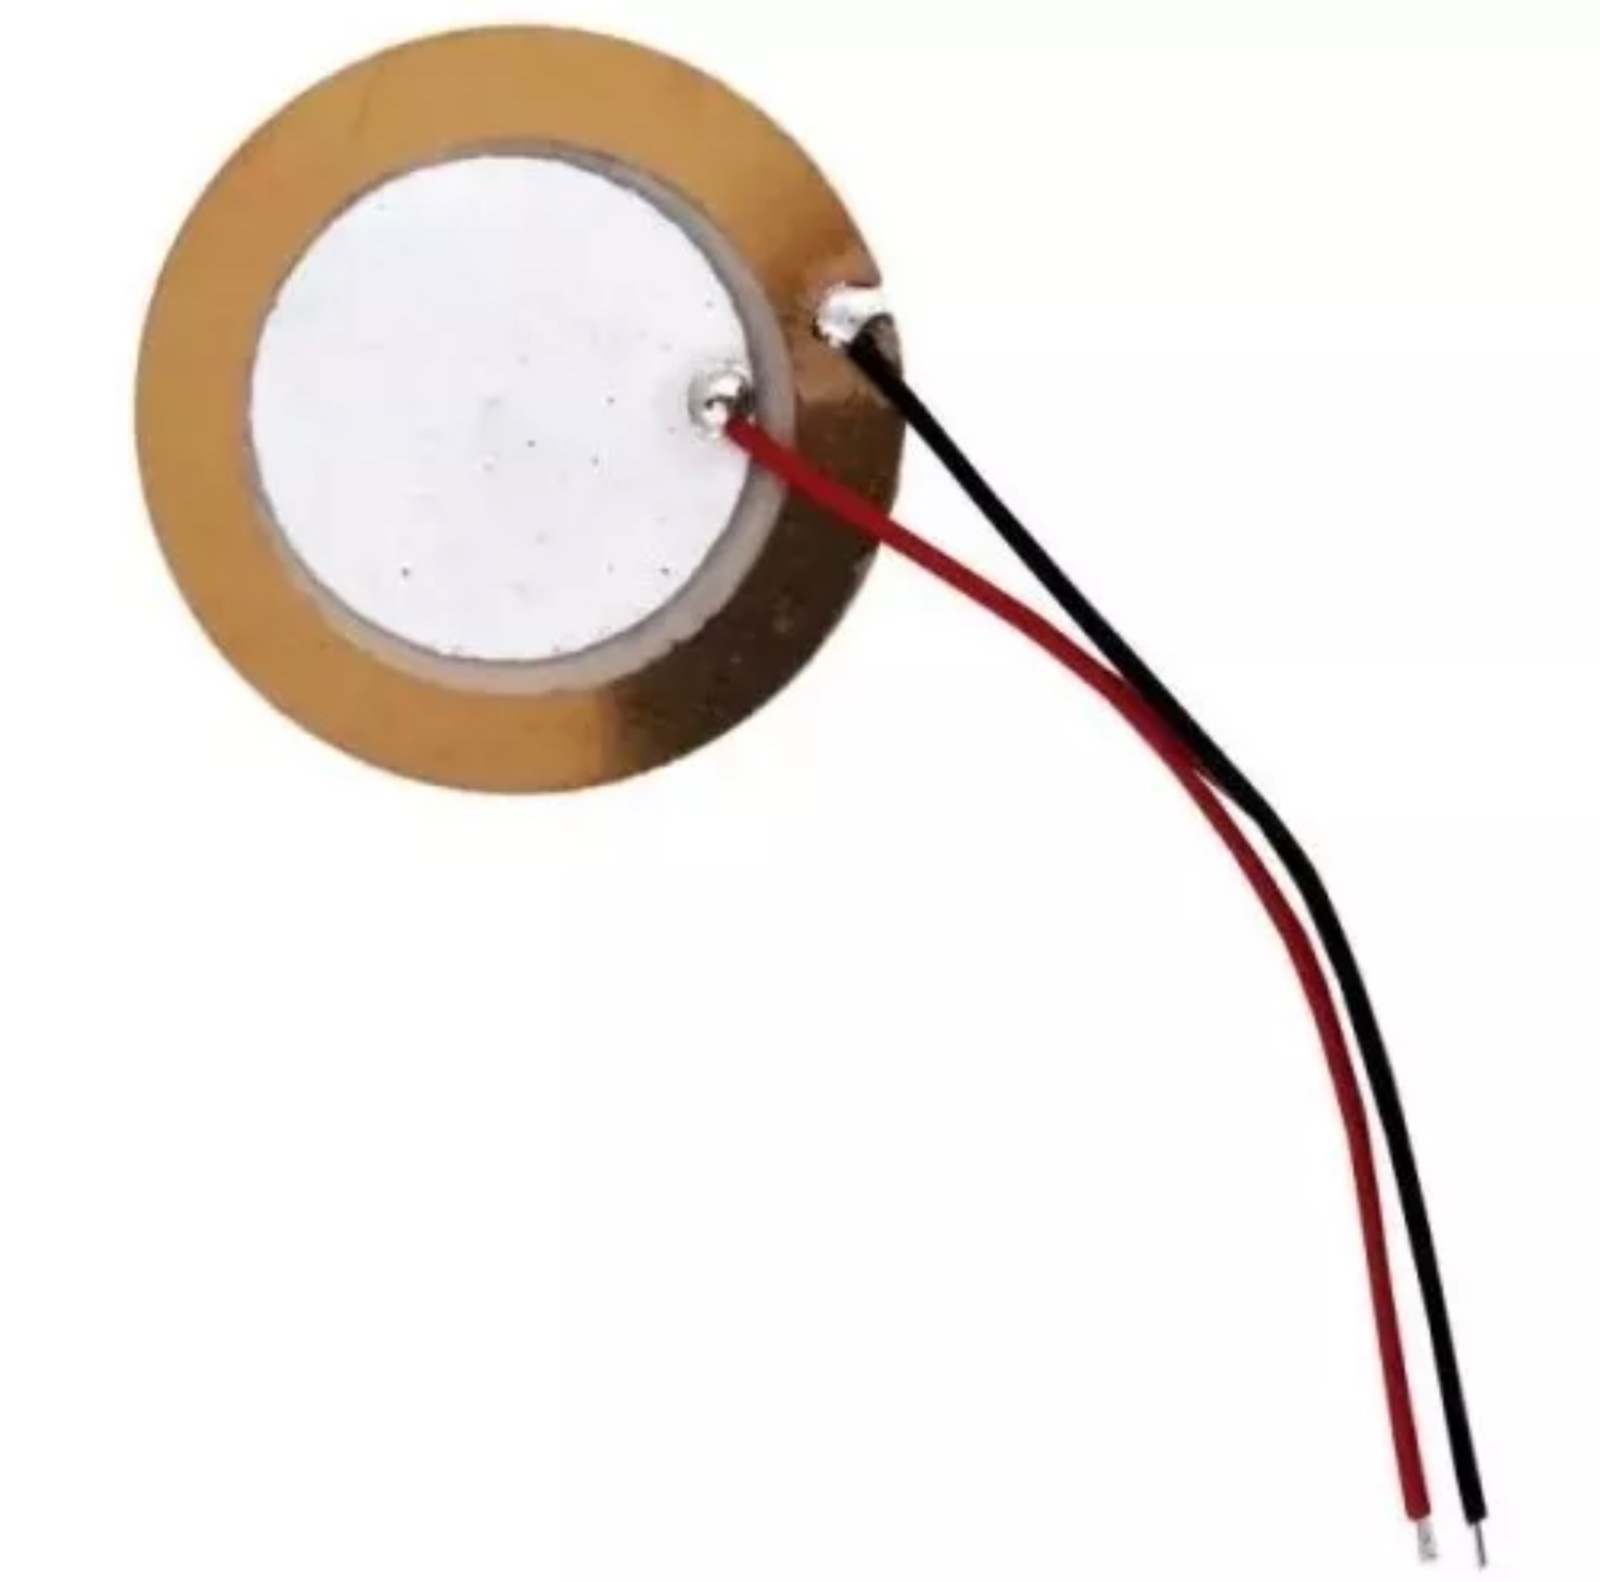
\includegraphics[width=0.15\textwidth]{img/Sensor_piezoelectrico}%
		\label{fig:piezoelectrico}
	}
	\subfloat[Funcionamiento de sensor piezoeléctrico]{%
		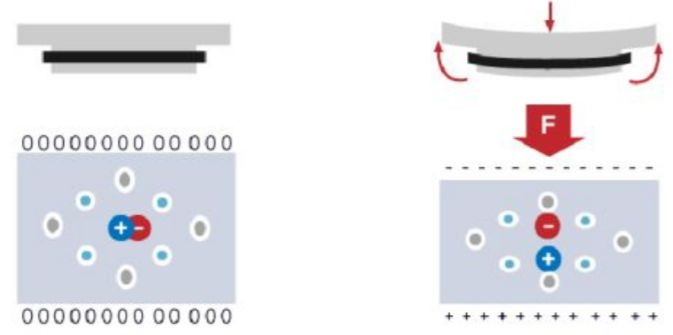
\includegraphics[width=0.3\textwidth]{img/piezoelectrico-fn}%
		\label{fig:piezoelectrico-fn}
	}
	\caption{Ejemplo de un sensor piezoeléctrico y su funcionamiento.}
	\label{fig:piezoelectricos}
\end{figure*}




\subsection{Interruptores de Efecto Hall}
Los interruptores de efecto Hall son dispositivos que detectan campos magnéticos y se utilizan para medir la posición o la velocidad de un objeto. A diferencia de los interruptores mecánicos, estos dispositivos no tienen partes móviles, lo que los hace más duraderos y confiables \cite{EfectoHall}.

En la \autoref{fig:interruptordeefectohall} se muestra un ejemplo de este sensor.

\begin{figure}[h!]
	\centering
	\subfloat[Interruptor de Efecto Hall]{%
		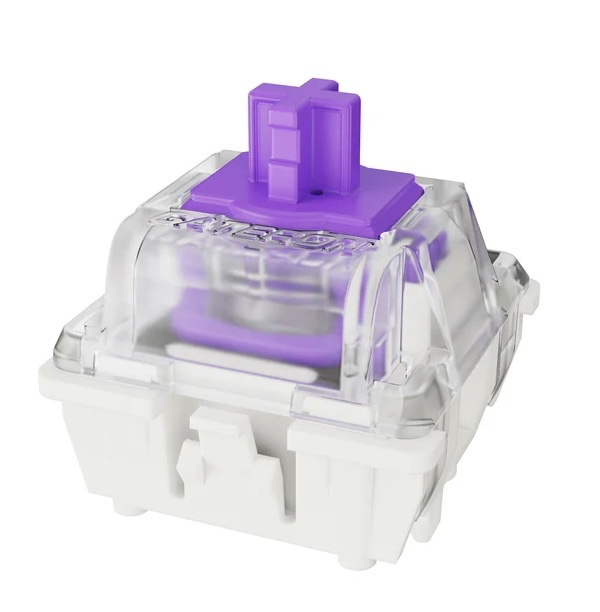
\includegraphics[width=0.15\textwidth]{img/Interruptor_efecto_Hall}%
		\label{fig:Interruptor_efecto_Hall}
	}
	\subfloat[Funcionamiento de Interruptor de Efecto Hall]{%
		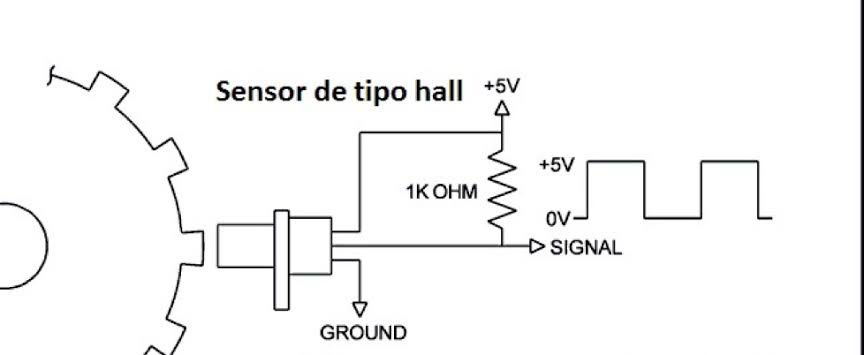
\includegraphics[width=0.35\textwidth]{img/Interruptor_efecto_Hall-fn}%
		\label{fig:Interruptor_efecto_Hall-fn}
	}
	\caption{Ejemplo de un interruptor de efecto Hall y su funcionamiento.}
	\label{fig:interruptordeefectohall}
\end{figure}
\section{Investigación}

\subsection{Giroscopio}
El giroscopio es un sensor que mide la velocidad angular en uno o más ejes, permitiendo detectar cambios en la orientación de un objeto. Este dispositivo es fundamental en aplicaciones que requieren estabilización y control de movimiento, como en cámaras, drones, sistemas de navegación inercial, videojuegos y dispositivos móviles \cite{MEMS}. Los giroscopios modernos, basados en tecnología MEMS (Micro-Electro-Mechanical Systems), son compactos, precisos y de bajo costo, lo que los hace ideales para su integración en sistemas robóticos y dispositivos portátiles.

En la \autoref{fig:giroscopio} se muestra un ejemplo de un giroscopio utilizado en aplicaciones de robótica y electrónica.

\begin{figure}[h]
	\centering
	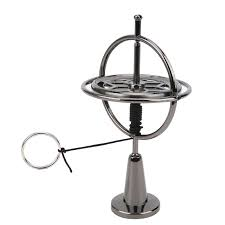
\includegraphics[width=0.3\linewidth]{img/Giroscopio}
	\caption{Ejemplo de un giroscopio utilizado en sistemas de navegación y estabilización.}
	\label{fig:giroscopio}
\end{figure}

\subsection{Acelerómetro}
El acelerómetro es un sensor que mide la aceleración lineal en uno o más ejes, permitiendo detectar movimientos, vibraciones e inclinaciones. Este dispositivo es ampliamente utilizado en teléfonos inteligentes, wearables, automóviles, drones y maquinaria industrial \cite{Acelerometro}. Los acelerómetros basados en tecnología MEMS son especialmente populares debido a su pequeño tamaño, bajo consumo de energía y alta precisión.

En la \autoref{fig:acelerometro} se muestra un ejemplo de un acelerómetro utilizado en aplicaciones de robótica y dispositivos móviles.

\begin{figure}[h]
	\centering
	\includegraphics[width=0.3\linewidth]{img/Acelerómetro}
	\caption{Ejemplo de un acelerómetro utilizado en sistemas de detección de movimiento.}
	\label{fig:acelerometro}
\end{figure}

\subsection{Magnetómetro}
El magnetómetro es un sensor que mide la intensidad y dirección de campos magnéticos, funcionando como una brújula digital. Este dispositivo es esencial en sistemas de navegación, donde se utiliza para determinar la orientación respecto al campo magnético terrestre. Además, los magnetómetros se emplean en aplicaciones de exploración geofísica, detección de metales y estudios de materiales magnéticos \cite{MEMS}.

En la \autoref{fig:magnetometro} se muestra un ejemplo de un magnetómetro utilizado en sistemas de navegación y exploración.

\begin{figure}[h]
	\centering
	\includegraphics[width=0.3\linewidth]{img/Magnetómetro}
	\caption{Ejemplo de un magnetómetro utilizado en sistemas de navegación y detección de campos magnéticos.}
	\label{fig:magnetometro}
\end{figure}

\subsection{LiDAR (Light Detection and Ranging)}
El LiDAR es una tecnología que mide distancias utilizando pulsos de luz láser, permitiendo generar mapas tridimensionales de alta precisión. Este sistema es ampliamente utilizado en vehículos autónomos para la detección de obstáculos y la navegación en entornos complejos. Además, el LiDAR se emplea en aplicaciones de cartografía, arqueología y estudios ambientales, donde es necesario obtener datos topográficos detallados \cite{LIDAR}.

En la \autoref{fig:lidar} se muestra un ejemplo de un sistema LiDAR utilizado en vehículos autónomos y aplicaciones de mapeo.

\begin{figure}[h]
	\centering
	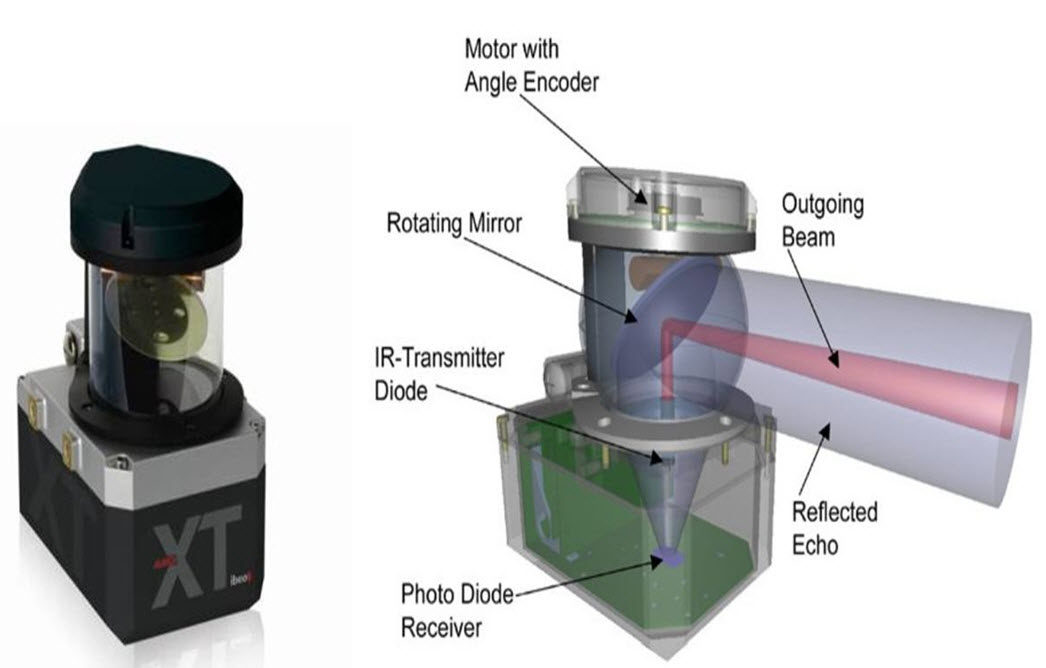
\includegraphics[width=0.5\linewidth]{img/LiDAR}
	\caption{Ejemplo de un sistema LiDAR utilizado en vehículos autónomos y cartografía.}
	\label{fig:lidar}
\end{figure}
\section{Conclusión} \label{sec:conclusion}
Solo añadan esta sección si lo consideran necesario. No es deben poner un resumen del contenido ni información importante que no se haya mencionado en una sección principal. Pueden poner la parte en la que más batallaron, el conocimiento más importante que consideran haber obtenido o algún comentario.
\subsection{Persona 1}
En caso de que haya sido una perspectiva individual, tienen que poner los comentarios de cada integrante y su nombre.
\subsection{Persona 2}
Esto me dará una retroalimentación desde la perspectiva de diferentes alumnos con diferentes roles.

%-------------------------------------------
% Bibliografía
%-------------------------------------------
\bibliographystyle{IEEEtran}  % Estilo de bibliografía IEEE
% La bibliografía se tomará del archivo "fuentes.bib"
\bibliography{fuentes}
	
\end{document}
